\section{Experiments}\label{sec:experiments}

We use the 15 layer convolutional architecture of \cite{zeiler2013visualizing}, trained on the
ImageNet 2012 dataset \cite{imagenet}.
The network contains 4 convolutional layers, 3 fully connected layers and a softmax output layer.
We evaluated the network on both CPU and GPU platforms. All measurements of prediction performance are with respect to the 20K validation images from the ImageNet12 dataset. 

We present results showing the performance of the approximations described in Section \ref{sec:approx_tech} in terms of prediction accuracy, speedup gains and reduction in memory overhead. 
All of our fine-tuning results were achieved by training with less than 2 passes using the ImageNet12 training dataset. 
Unless stated otherwise, classification numbers refer to those of fine-tuned models.
 
\subsection{Speedup}
The majority of forward propagation time is spent on the first two convolutional layers (see Supplementary Material for breakdown of time across all layers).
Because of this, we restrict our attention to the first and second convolutional layers in our speedup experiments. 
However, our approximations could easily
applied to convolutions in upper layers as well.

We implemented several CPU and GPU approximation routines 
in an effort to achieve empirical
speedups. Both the baseline and approximation CPU code is implemented
in C++ using Eigen3 library \cite{eigenweb} compiled with Intel MKL.
We also use Intel's implementation of openmp and multithreading. The
baseline gives comparable performance to highly optimized MATLAB
convolution routines and all of our CPU speedup results are computed
relative to this.  We used Alex Krizhevsky's CUDA convolution routines
\footnote{\url{https://code.google.com/p/cuda-convnet/}} as a baseline for GPU
comparisons. The approximation versions are written in CUDA. All GPU
code was run on a standard nVidia Titan card.

We have found that in practice it is often difficult to achieve
speedups close to the theoretical gains based on the number of
arithmetic operations (see Supplementary Material for discussion of theoretical gains).
Moreover, different computer architectures and CNN 
architectures afford different optimization strategies making most
implementations highly specific.  However, regardless of
implementation details, all of the approximations we present reduce
both the number of operations and number of weights required to
compute the output by at least a factor of two, often more.  

\subsubsection{First Layer}

The first convolutional layer has 3 input channels, 96
output channels and 7x7 filters.  We approximated the weights in this
layer using the monochromatic approximation described in Section
\ref{subsec:monochromatic}. The monochromatic approximation works well if
the color components span a small number of one dimensional
subspaces. Figure \ref{fig:RGB_components} illustrates the effect of the monochromatic approximation on the first layer filters. 
%Interestingly, we
%notice that the approximated filters often appear to be cleaned up
%versions of the original filters. This leads up to believe that the
%approximation techniques presented here might be viable strategies of
%cleaning up or denoising weights after training, potentially improving generalization performance.

\begin{figure}[t]
\centering
\begin{minipage}{\textwidth}
	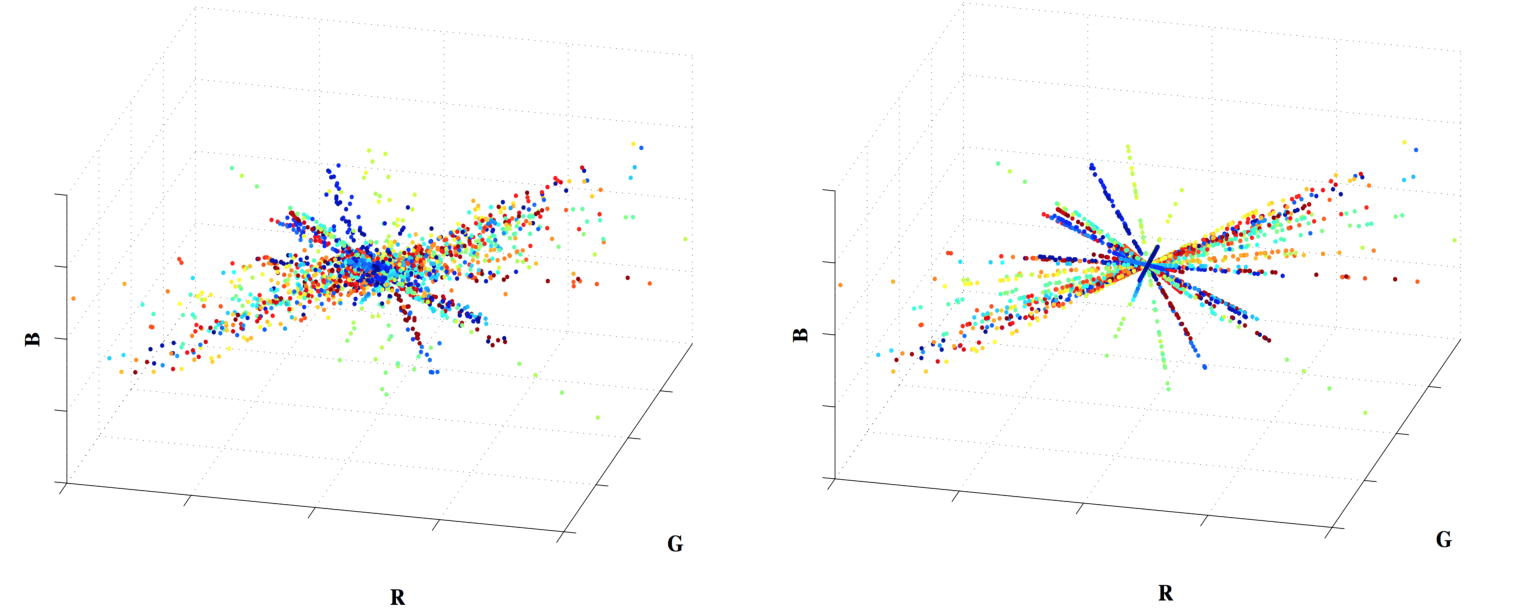
\includegraphics[width=0.55\linewidth]{img/RGB_components_stacked.pdf}
	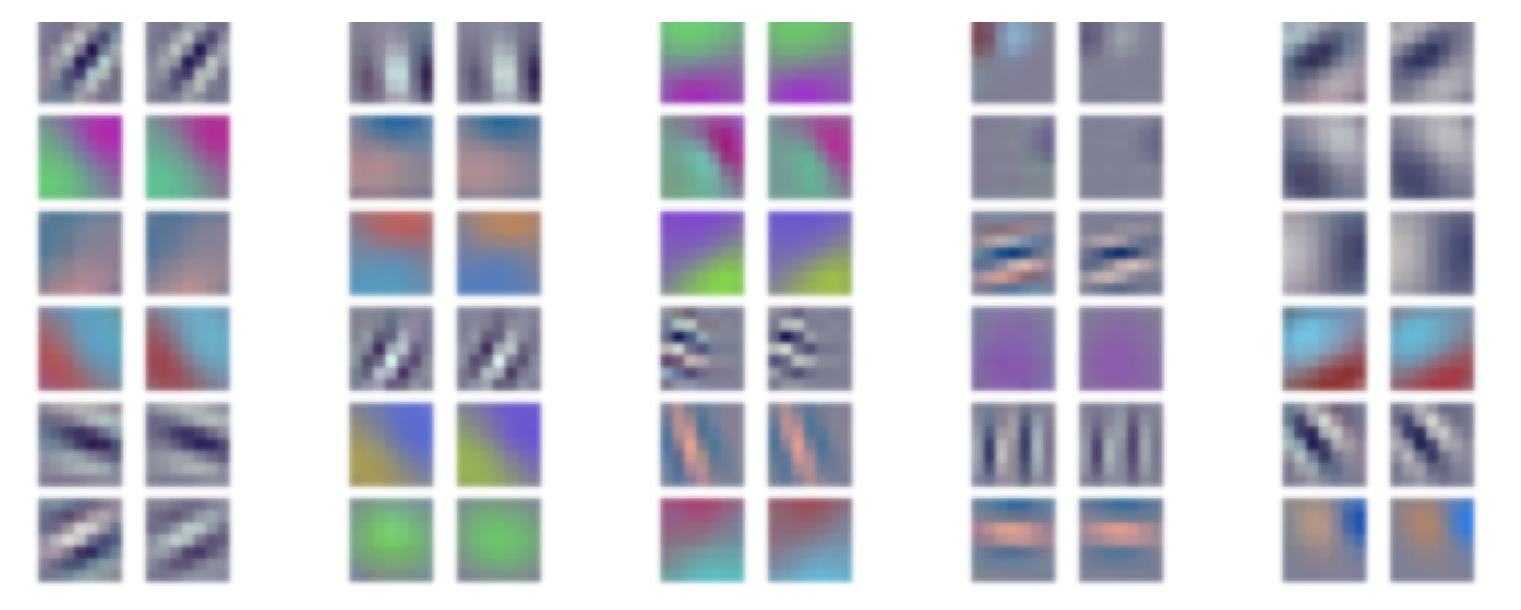
\includegraphics[width=0.45\linewidth]{img/denoised_stacked.pdf} 
\end{minipage}
\vspace{-3mm}
\label{fig:RGB_components}
\caption{Visualization of the 1st layer filters. {\bf (Left)} Each component of the 96 7x7 filters is plotted in RGB space. Points are colored based on the output filter they belong to. Hence, there are 96 colors and $7^2$ points of each color. Leftmost plot shows the 
  original filters and the right plot shows the filters after the monochromatic approximation, where each filter has been projected down to a line in colorspace. {\bf (Right)} Original and approximate versions of a selection of 1st layer filters.}
\vspace{-3mm}
\end{figure}

%We evaluated the network on 20K validation images from the ImageNet12 dataset using various monochromatic approximations for the first layer weights. 
The only parameter in the approximation is $C'$, the number of color channels used for the intermediate representation. As expected, the network performance begins to degrade as $C'$ decreases. 
The number of floating point operations required to compute the output of the monochromatic convolution is reduced by a factor of $2-3\times$, with the larger gain resulting for small $C'$. 
%Since the majority of the operations result from the convolution part of the computation, rather than the color transform,
%the theoretically achievable speedup decreases only slightly as $C'$ is increased.
%In practice, we found it difficult to optimize the monochromatic convolution routines as for large $C'$ since less work can be shared amongst output filters making it challenging to parallelize.
Figure \ref{fig:mono_speedups} shows the empirical speedups we achieved on CPU and GPU and the corresponding network performance for various numbers of colors used in the monochromatic approximation.   
Our CPU and GPU implementations achieve empirical speedups of $2-2.5\times$ relative to the baseline with less than 1\% drop in classification performance. 

\begin{figure}[t]
\centering
\begin{minipage}{0.9\textwidth}
      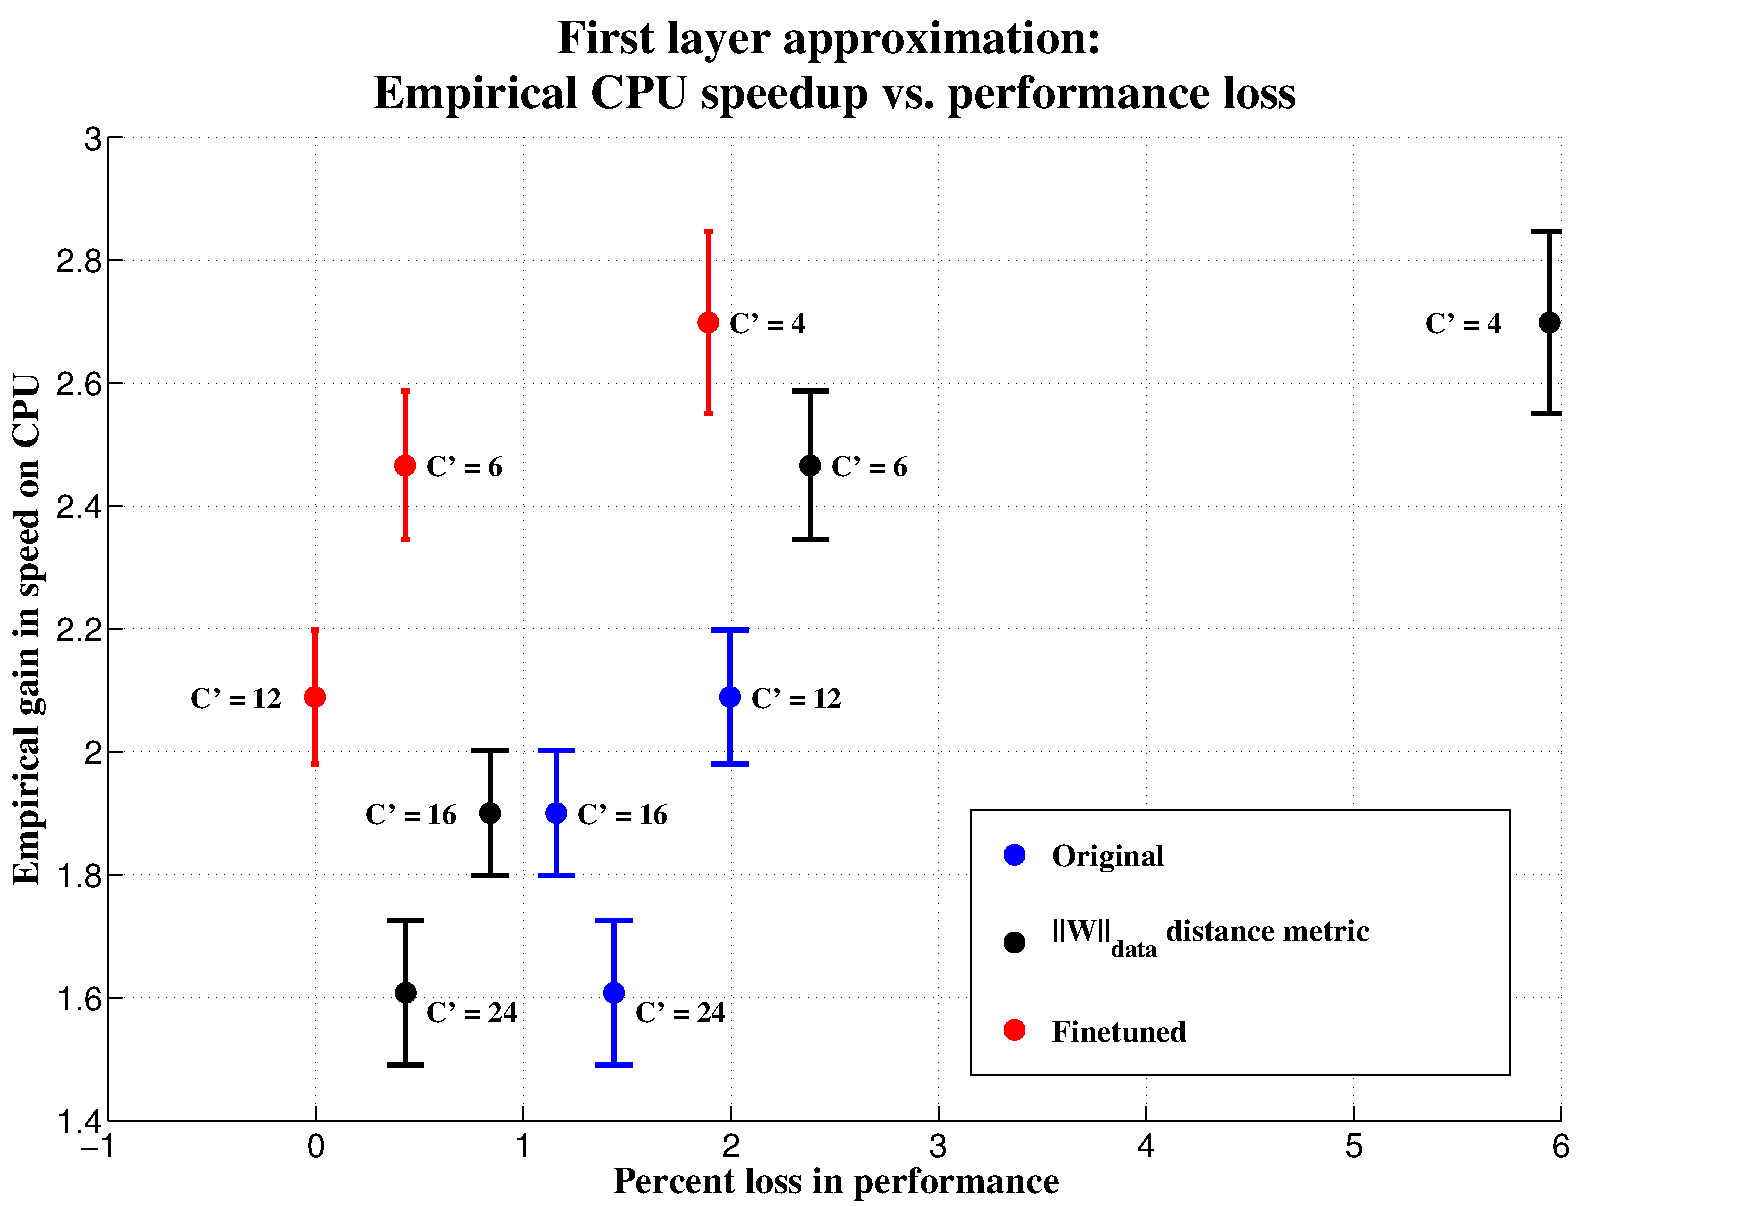
\includegraphics[width=0.5\linewidth]{img/layer1_CPUspeedup_vs_performance_loss_finetune_and_orig.pdf}
	\quad
      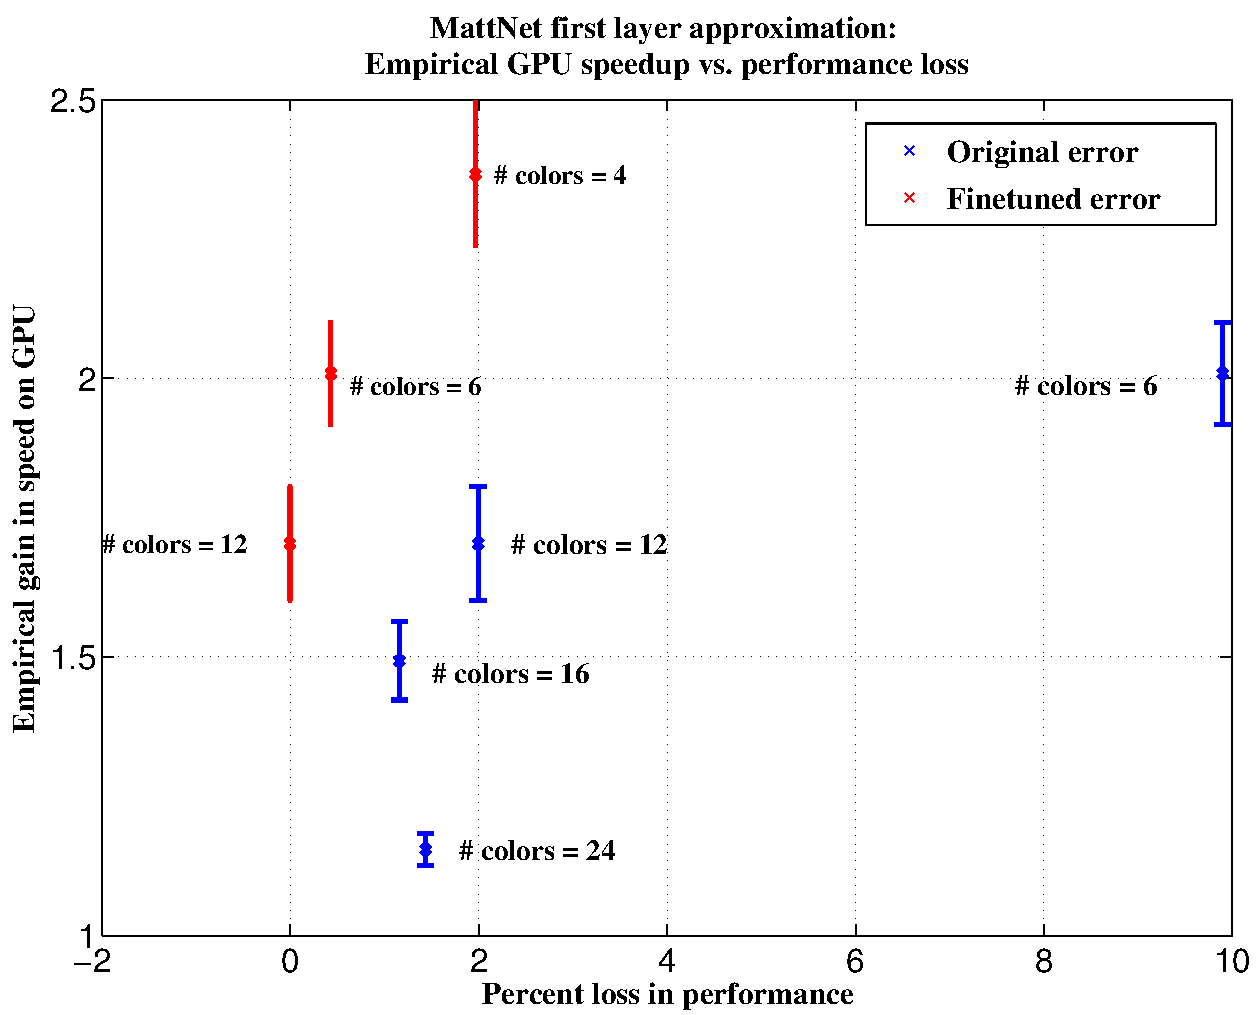
\includegraphics[width=0.5\linewidth]{img/layer1_GPUspeedup_vs_performance_loss_finetune_and_orig.pdf}
\end{minipage}
\caption{Empirical speedups on ({\bf Left}) CPU and ({\bf Right}) GPU for the first layer. $C'$ is the number of colors used in the approximation.}
\label{fig:mono_speedups}
\end{figure}

\subsubsection{Second Layer}
The second convolutional layer has 96 input channels, 256 output channels and 5x5 filters. 
We approximated the weights using the techniques described in Section \ref{subsec:clustering}. 
We explored various configurations of the approximations by varying the number of input clusters $G$, the number of output clusters $H$ and the rank of the approximation (denoted by $K_1$ and $K_2$ for the SVD decomposition and $K$ for the outer product decomposition). 

Figure \ref{fig:biclust_speedups} shows our empirical speedups on CPU
and GPU and the corresponding network performance for
various approximation configurations. For the CPU implementation we used the biclustering with SVD approximation. For the GPU implementation we using the biclustering with outer product decomposition approximation.  
We achieved promising results and present speedups of $2-2.5\times$ relative to the baseline with less than a 1\% drop in performance.

\begin{figure}[t]
\centering
\begin{minipage}{0.9\textwidth}
      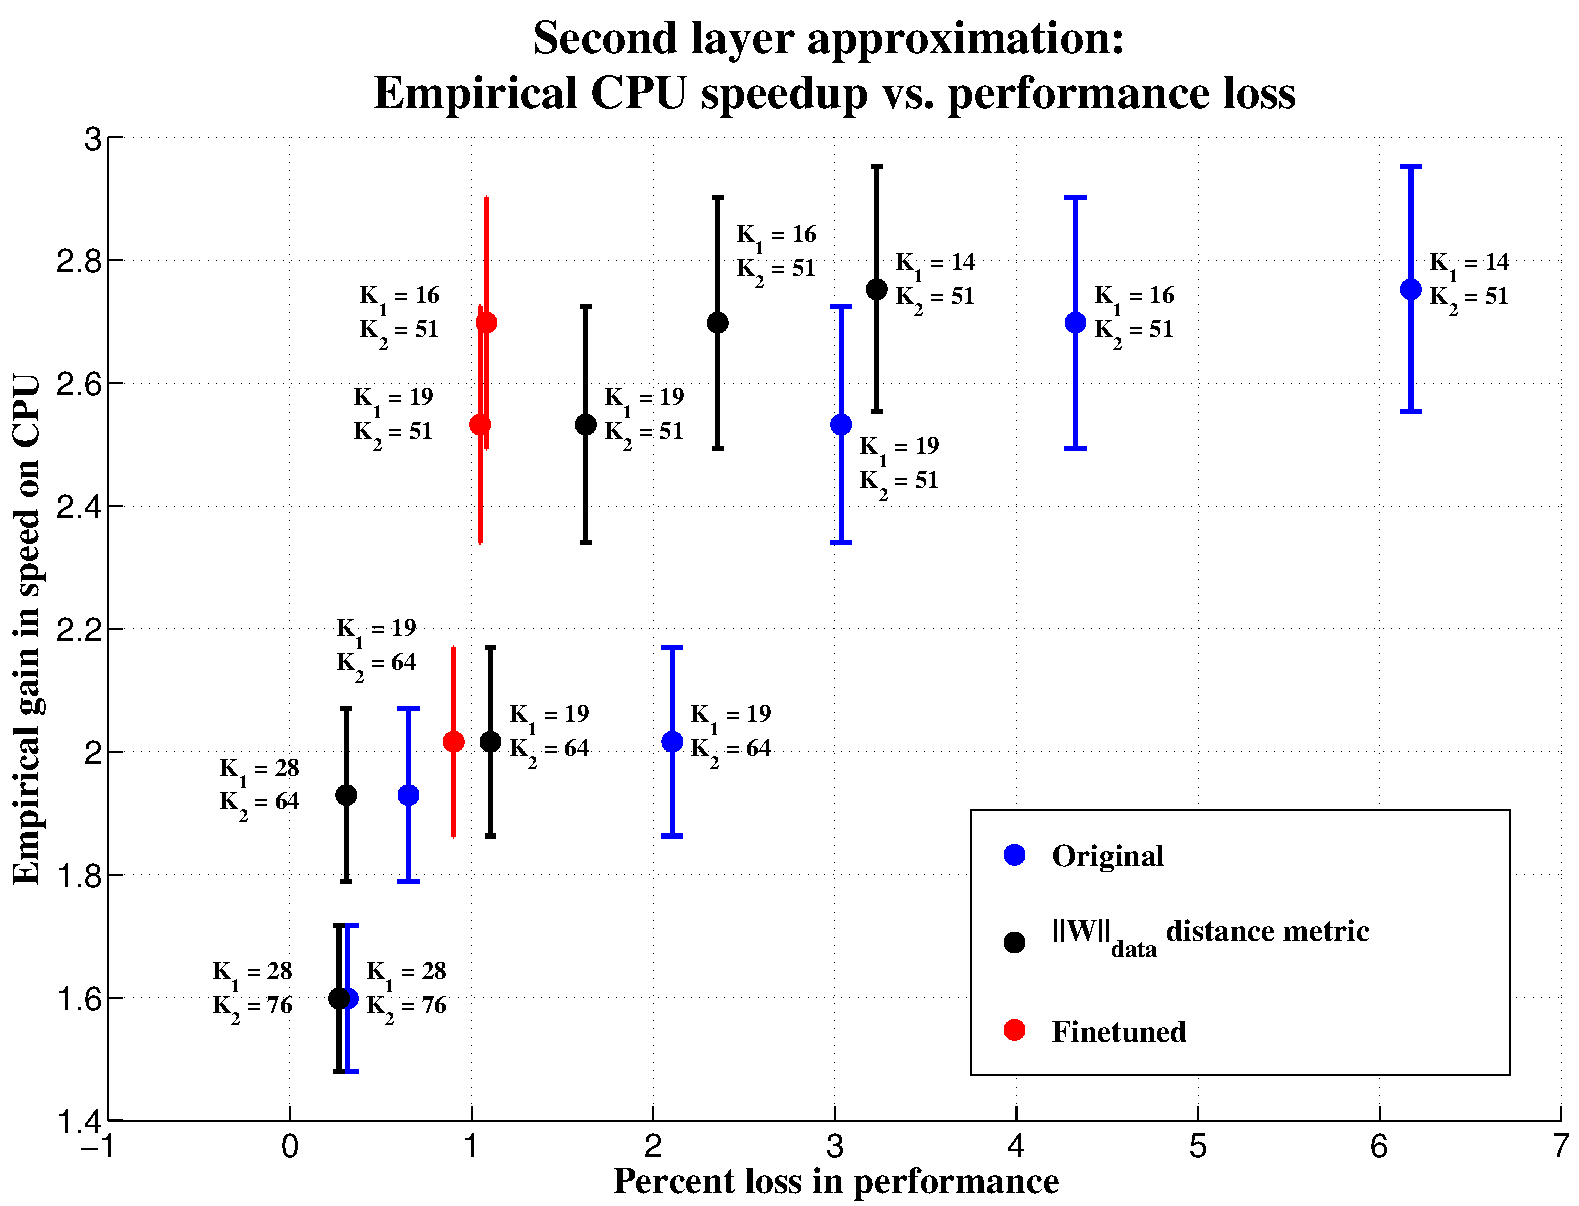
\includegraphics[width=0.5\linewidth]{img/layer2_CPUspeedup_vs_performance_loss_finetune_and_orig.pdf}
      \quad
      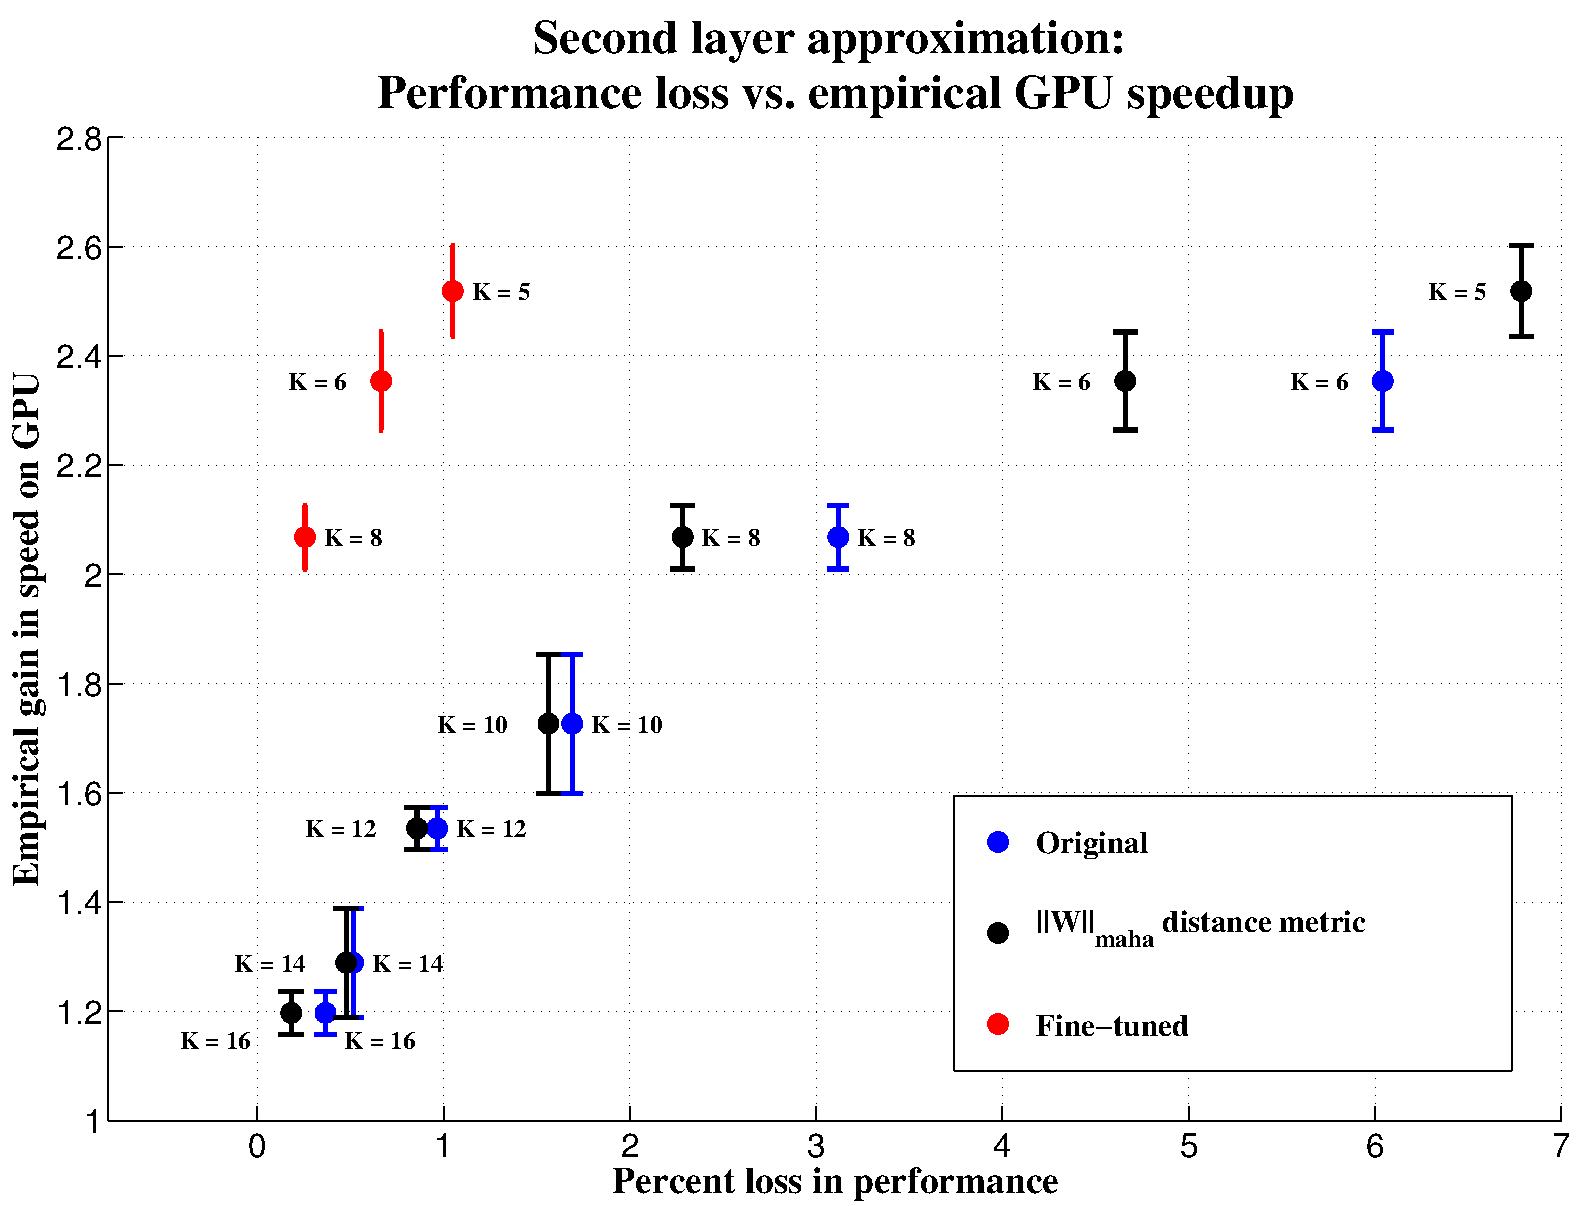
\includegraphics[width=0.5\linewidth]{img/layer2_GPUspeedup_vs_performance_loss_finetune_and_orig.pdf}
\end{minipage}
\caption{Empirical speedups for second convolutional layer. ({\bf Left}) Speedups on CPU using biclustered ($G = 2$ and $H = 2$) with SVD approximation. ({\bf Right}) peedups on GPU using biclustered ($G = 48$ and $h = 2$) with outer product decomposition approximation.}
\label{fig:biclust_speedups}
\end{figure}

\subsection{Combining approximations}
The approximations can also be cascaded to provide greater speedups.
The procedure is as follows. 
Compress the first convolutional layer weights and then 
fine-tune all the layers above until performance is restored. 
Next, compress the second convolutional layer weights that result from the fine-tuning.
Fine-tune all the layers above until performance is restored and then continue the process. 

We applied this procedure to the first two convolutional layers. 
Using the monochromatic approximation with 6 colors for the first layer and the biclustering with outer product decomposition approximation for the second layer ($G = 48; H = 2; K = 8$) and 
fine-tuning with a single pass through the training set we are able to keep accuracy within 1\% of the original model.
This procedure could be applied to each convolutional layer, in this sequential manner, to achieve overall speedups much greater than any individual layer can provide. 
A more comprehensive summary of these results can be found in the Supplementary Material.

\subsection{Reduction in memory overhead}
In many commercial applications memory conservation and storage are a
central concern. This mainly applies to embedded systems
(e.g. smartphones), where available memory is limited, and users are
reluctant to download large files. In these cases, being able to
compress the neural network is crucial for the viability of the
product. 

In addition to requiring fewer operations, our approximations
require significantly fewer parameters when compared to the original
model. 
Since the majority of parameters come from the fully connected layers, we include these layers in our analysis of memory overhead. 
We compress the fully connected layers using standard SVD as described in \ref{subsubsec:svd_tensor}, using $K$ to denote the rank of the approximation.
 
Table \ref{table:memory} shows the number of parameters for
various approximation methods as a function of hyperparameters for the approximation techniques.
The table also shows the empirical reduction of parameters and the corresponding network performance for specific instantiations of the approximation parameters.

\begin{table}[t]
\tiny
\centering
\begin{tabular}{|l|c|c|c|c|}
\hline
{\bf Approximation method} & {\bf Number of parameters} & {\bf Approximation} & {\bf Reduction} & {\bf Increase }\\ 
& & {\bf hyperparameters} &  {\bf in weights} & {\bf in error}\\
\hline
\hline
Standard colvolution & $CXYF$ & & &\\
\hline
Conv layer 1: Monochromatic & $CC' + XYF$ & $C' = 6$ & $3\times$ & 0.43\%\\
\hline
Conv layer 2: Biclustering & $GHK (\frac{C}{G} + XY + \frac{F}{H})$ & $G = 48$; $H = 2$; $K = 6$ & 5.3$\times$ & 0.68\%\\
	    + outer product decomposition  & &  & &\\
\hline
Conv layer 2: Biclustering + SVD& $G H (\frac{C}{G}K_1 + K_1 X Y K_2 + K_2 \frac{F}{H})$ & $G = 2; H = 2$; $K_1 = 19$; $K_2 = 24$ & $3.9\times$ & 0.9\% \\
\hline
Standard FC & $N M$ & & &\\
\hline
FC layer 1: Matrix SVD & $NK + KM$ & $K = 250$ & $13.4\times$ & 0.8394\%\\
                      & & $K = 950$ & $3.5\times$ & 0.09\%\\
\hline 
FC layer 2: Matrix SVD & $NK + KM$ & $K = 350 $ & $5.8\times$ & 0.19\%\\
                      & & $K = 650$ & $3.14\times$ & 0.06\%\\
\hline 
FC layer 3: Matrix SVD & $NK + KM$ & $K = 250$ & $8.1\times$ & 0.67\%\\
                      & & $K = 850$ & $2.4\times$ & 0.02\%\\
\hline 
\end{tabular}
\caption{Number of parameters expressed as a function of hyperparameters for various approximation methods and empirical reduction in parameters with corresponding network performance.} 
\label{table:memory}
\vspace{-3mm}
\end{table}
\vspace{-3mm}
